\section{Cross-Metric Agreement on the OLMo-2-7B RLHF Experiment}\label{app:rlhf-cross-metric}

The RLHF case study (Section~\ref{sec:rlhf-experiment}) reports the headline monotone $D_{Ca_n}$ drop in Table~\ref{tab:rlhf-diversity} and Figure~\ref{fig:rlhf-ak-violin}.
Figure~\ref{fig:rlhf-metric-scatter} plots $D_{Ca_n}$ against the lexical (EAD) and semantic (SentBERT) baselines on the same length-matched subset, confirming that the three metrics see the same diversity-loss signal.

\IfFileExists{../figures/rlhf_experiment/metric_correlation_scatter_alpacaeval_lm.pdf}{%
\begin{figure*}[!htbp]
\centering
\begin{subfigure}[t]{\textwidth}
    \centering
    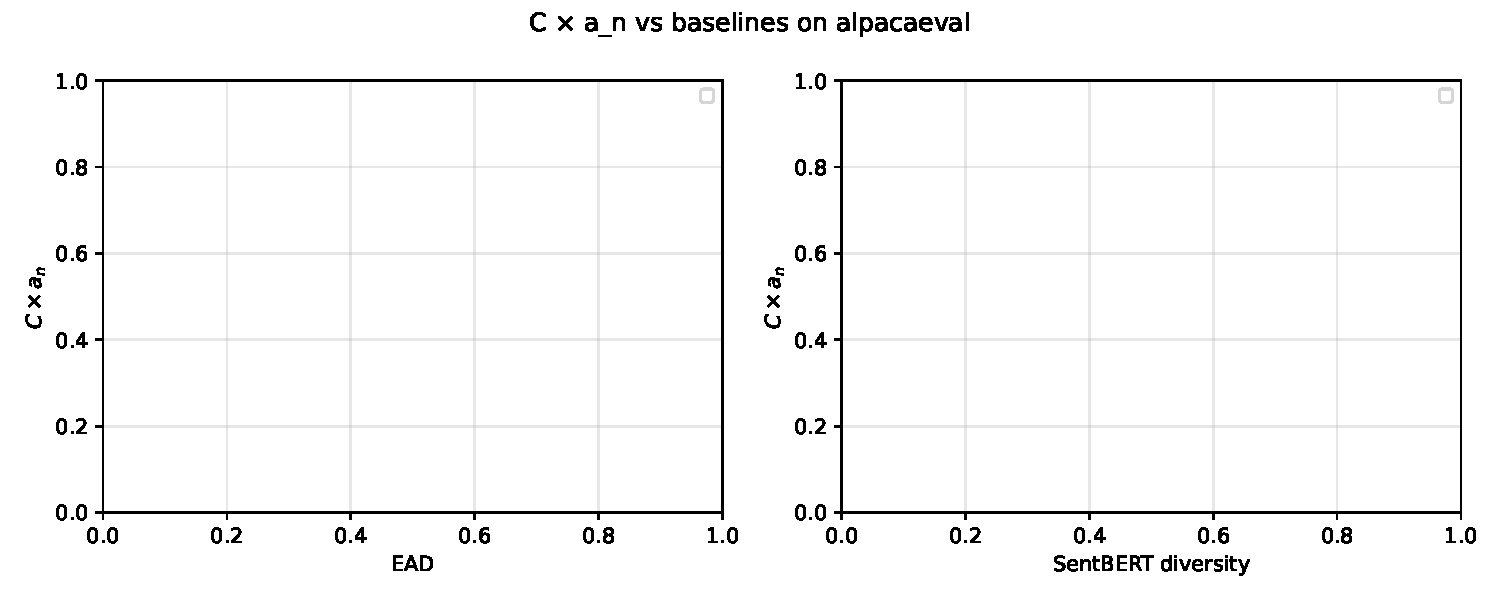
\includegraphics[width=0.85\textwidth]{../figures/rlhf_experiment/metric_correlation_scatter_alpacaeval_lm.pdf}
    \caption{AlpacaEval (length-matched, $n=\olmoLmAlpacaN$ prompts).}
\end{subfigure}\\[0.5em]
\begin{subfigure}[t]{\textwidth}
    \centering
    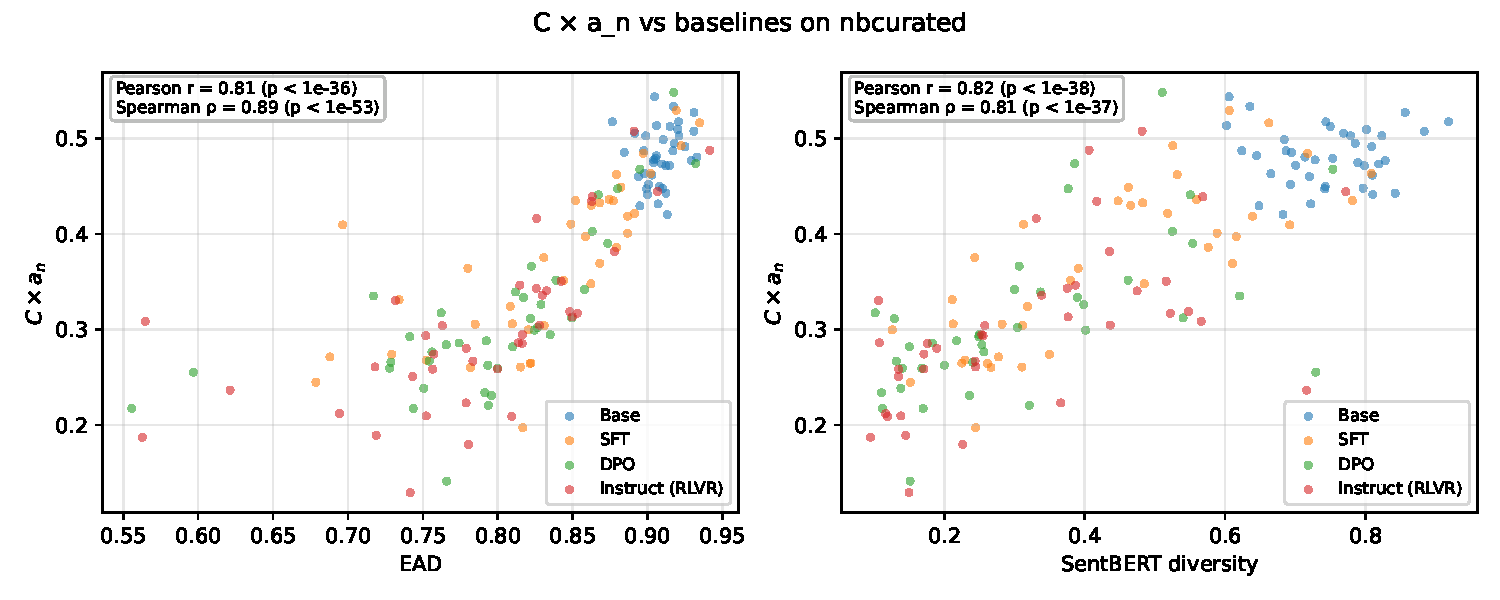
\includegraphics[width=0.85\textwidth]{../figures/rlhf_experiment/metric_correlation_scatter_nbcurated_lm.pdf}
    \caption{NoveltyBench curated (length-matched, $n=\olmoLmNbCuratedN$ prompts).}
\end{subfigure}
\caption{Per-prompt $D_{Ca_n}$ versus EAD (left subpanel) and SentBERT-similarity diversity (right subpanel), coloured by stage, on the length-matched subset of prompts. Length-matching truncates each (stage, prompt) tuple's responses to a common per-prompt byte budget so the per-byte conditional surprise that defines $a_n$ is not depressed by response length. Pearson $r$ and Spearman $\rho$ (two-sided $p$) are reported in each panel. The rank correlations are positive across both prompt sets and both baselines: $D_{Ca_n}$ tracks the same diversity-loss signal EAD and SentBERT detect, and the agreement is not an artefact of response length.}
\label{fig:rlhf-metric-scatter}
\end{figure*}
}{}
